Il dataset è formato da numeri in formato float, ma in alcuni casi si hanno dei NaN o dei \textit{inf}. Occorre quindi sistemare il dataset.\\
\begin{lstlisting}
brain_tumor_data = pd.read_csv(r"Data/bt_dataset_t3.csv")

del brain_tumor_data["Image"]
brain_tumor_data = brain_tumor_data.replace(np.inf, 999)
bt_rep = brain_tumor_data.mean()
brain_tumor_data = brain_tumor_data.fillna(bt_rep)

brain_tumor_data.to_csv(r"Data/bt_dataset_t3_fixed.csv")
\end{lstlisting}

Mediante il modulo Pandas si va a leggere il file csv che costituisce il dataset e lo si trasforma in un \textit{dataframe}, in modo da poter eseguire le operazioni di preprocessing. La trasformazione in dataframe verrà eseguita in ogni algoritmo per poter eseguire le tecniche di classificazione.\\
Per i dati inf indicano un valori che tendono a infinito. Per mantenere la loro caratteristica si è pensato di sostituire i dati di tipo inf con un valore molto alto, ad esempio 999.
\begin{lstlisting}
brain_tumor_data = brain_tumor_data.replace(np.inf, 999)
\end{lstlisting}
I dati NaN sono dati che non si hanno in possesso. L'idea è quindi quella di renderli influenti negli algoritmi, perciò può essere una buona idea sostituirli con la media della colonna (feature).
\begin{lstlisting}
bt_rep = brain_tumor_data.mean()
\end{lstlisting}
Infine con l'istruzione di Pandas \textit{to\_csv()} si salvano tali operazioni in un nuovo csv che costituirà il dataset aggiustato. Il nuovo csv verrà utilizzato come input negli algoritmi che implementano le tecniche di classificazione. In questo modo si evitano errori legati all'inconsistenza dei dati.
\begin{figure}[!htb]
	\minipage{0.45\textwidth}
	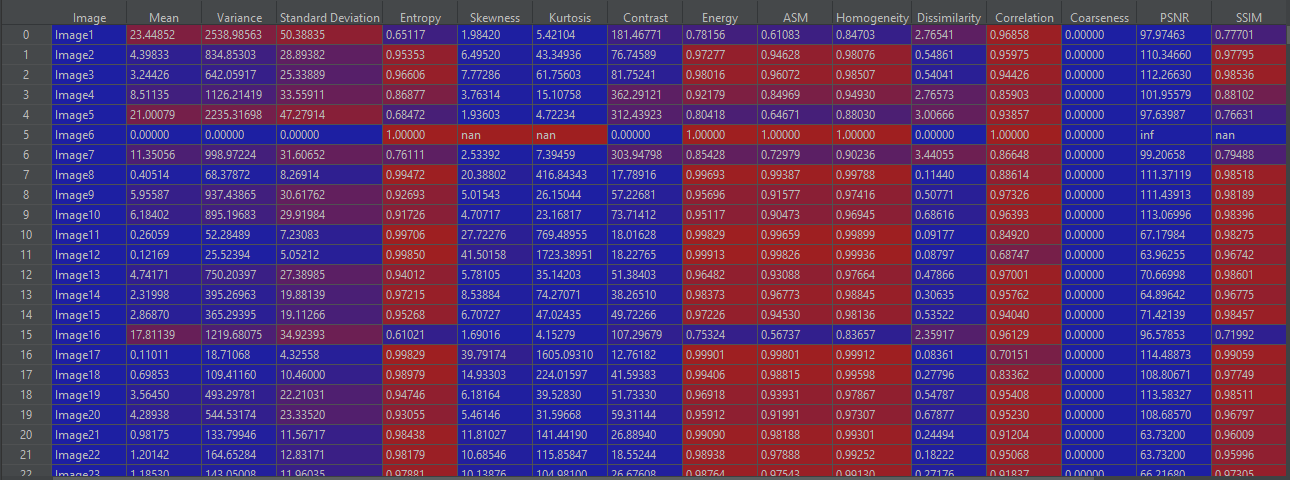
\includegraphics[width=1.2\linewidth]{image/braintumordataset.png}
	\label{fig:immagine01}
	\endminipage\hfill
	\minipage{0.45\textwidth}
	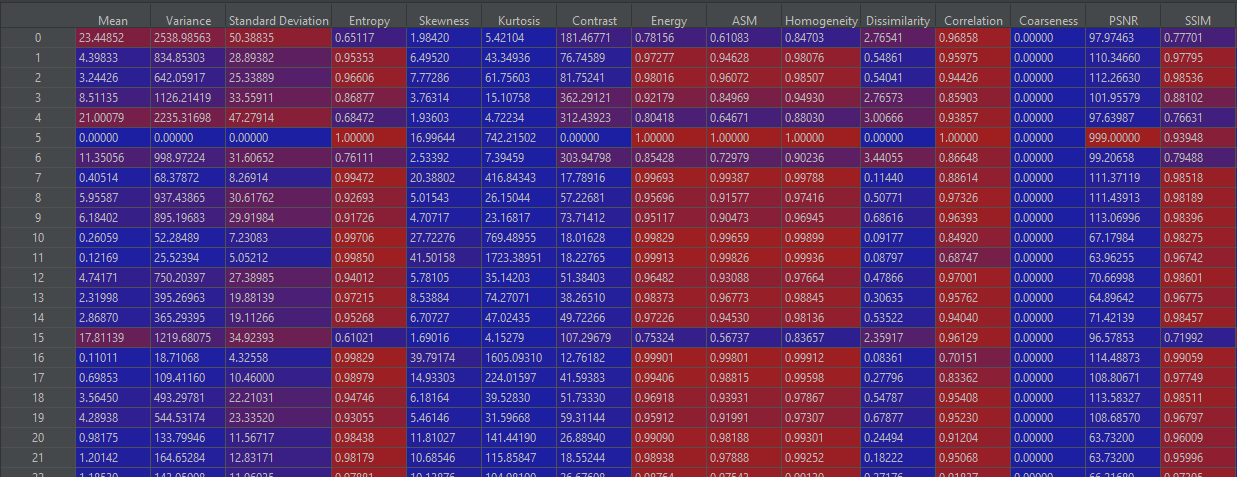
\includegraphics[width=1.2\linewidth]{image/braintumordatasetfixed.png}
	\label{fig:immagine2}
	\endminipage
	\caption{A sinistra il dataframe con dati inconsistenti, a desta il dataframe fixato.}
\end{figure}
\newpage
L'IDE utilizzato è \textit{PyCharm} e grazie al suo comodo strumento di debugging è stato semplice visualizzare la struttura del dataframe e quindi valutare il corretto funzionamento del codice. 